% document style header
\documentclass[a4paper, 12pt]{config/homework}

% import default packages
\usepackage{config/defpackages}
% import custom math commands
\usepackage{config/domath}
% for inserting pages
\usepackage{pdfpages}

% end preamble
\begin{document}

% document title
\noindent
\begin{tabularx}{\textwidth}{>{\centering\arraybackslash}X>{\centering\arraybackslash}X>{\centering\arraybackslash}X}
Calvin Sprouse & PHYS489 1A & 2024 Jan 12\\
\midrule
\end{tabularx}

% reflection
% Select and write a reflection on a graded artifact (e.g., homework assignment, test, report) from a 300- or 400-level required physics course that you think best demonstrates the learning outcome of knowing key physical concepts and applying them to analyze and interpret the behavior of physical systems. The artifact you select should be from an upper division physics class that is required in your physics degree program. Response should be 1/2 page.

The artifact I selected is a particular homework assignment from PHYS383 Electromagnetic Theory 3 taken Spring 2023. I selected this assignment not because it is my best preforming, I got a 29/30, or most challenging, but because I remember working on this assignment with joy. This is also around the time I felt that my time-consuming challenge of using \LaTeX\ to prepare my homework was finally paying off and improving the way I did physics. Typesetting my homework has enabled me to use more explanation in my work which not only serves to demonstrate my knowledge but helped me understand the process of doing physics. Throughout this assignment I am utilizing Maxwell's equations, vector calculus, and a healthy dose of appropriate approximations to understand relativity in the context of Electromagnetic Theory. Problem 2 in particular is concerned with arriving at the precursor to relativity through an understanding of how information on electromagnetic systems takes time to propagate. I am also able to leverage this understanding of physical systems, and a healthy dose of approximations, in problem 3 to explore signal radiation. Most important to me, however, is the theoretical understanding explored in problem 1. The determination of gauge in an electromagnetic system reveals a lot of information about the system before a particular solution is found. The problem of determining gauge shows up frequently in electromagnetic theory and understanding how to work with a gauge is an important precursor to physics theory. While this is not my most perfect assignment nor most challenging I feel this represents my understanding of key concepts, my ability to apply them, and my desire to take my education further.

% insert artifact page
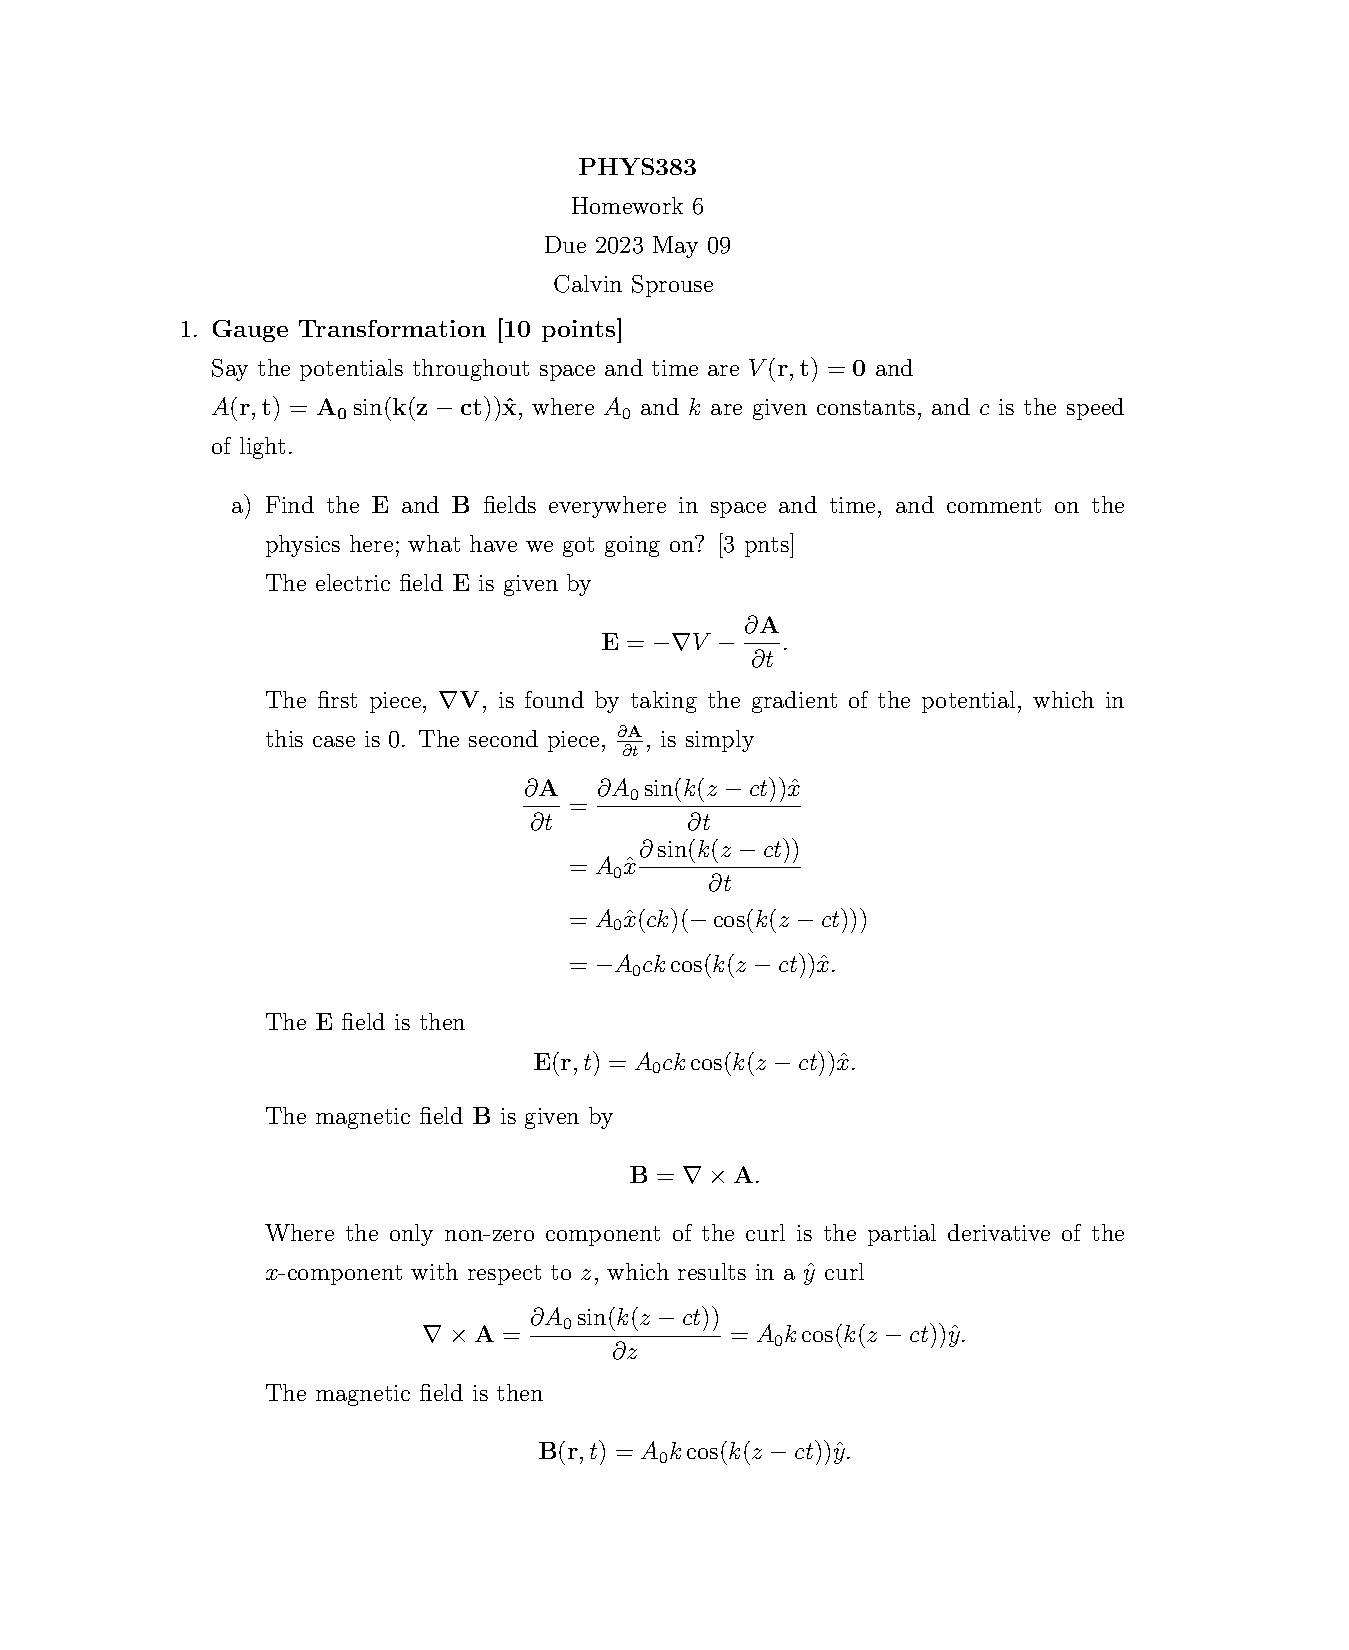
\includepdf[pages=-]{em_hw_6.pdf}

\end{document}
